\documentclass{article}

\usepackage[utf8]{inputenc}
\usepackage{graphicx}
\usepackage{amsmath}
\usepackage[letterpaper, portrait, margin=1in]{geometry}
\usepackage{gensymb}
\title{Molecules and Cells HW 6}
\date{October 6th, 2016}

\begin{document}

\maketitle

1. \begin{figure}[h]
  \centering
 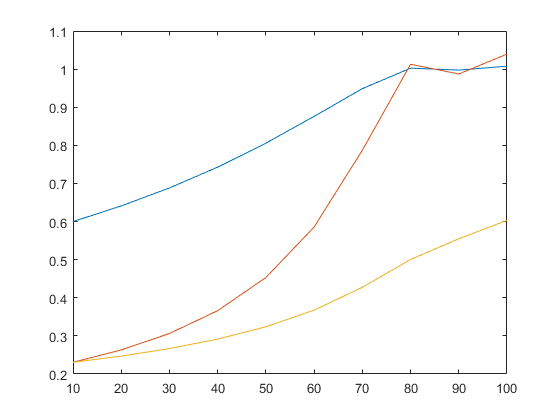
\includegraphics[scale=0.5]{P1.png}
\end{figure}


2a. Increase. Without the repressor gene, the trp operon will be active regardless of whether or not tryptophan is present. Even at high concentrations of tryptophan, the operon will still be active.

2b. Because the gene making the repressor gene is not located in the trp operon, this is a trans mutation

2c. Yes, it can be fixed because it is a trans mutation.
\vspace{5mm}

4. One thing to note is that many regulatory proteins are controlled by internal and external conditions. For examples, the presence or absence of hormones like cortisol may activate or deactivate the expression of certain regulatory proteins. In addition to this, regulatory proteins are often interconnected, so one regulatory protein might prevent a protein from being expressed while also activating the expression of a third one, which then goes back and regulates the first regulatory protein.
\vspace{5mm}

4. (D) $K_m$ is the concentration at which the rate is half of $V_{max}$. A smaller $K_m$ will mean a smaller concentration to reach $V_{mx}$.
\vspace{5mm}

5. (E)
\vspace{5mm}

6a. I

6b. D

6c. I

6d. NC

6e. I

6f. NC

6g. I

6h. I
\end{document}